\documentclass{article}
\usepackage{graphicx}
\usepackage[margin=1.5cm]{geometry}
\usepackage{amsmath}
\usepackage{hyperref}

\begin{document}

\title{Week 11 Writing Activity: Writing Mechanics in Essays and Articles and Chapter 8 of \textit{The Scientific Attitude}}
\author{Prof. Jordan C. Hanson (INTD100)}

\maketitle

\section{Links for Today}
\small
\begin{enumerate}
\item
\begin{verbatim}
https://www.npr.org/2015/12/09/459026242/scientific-evidence-doesn-t-support-global-warming-sen-ted-cruz-says
\end{verbatim}
\item
\begin{verbatim}
https://www.commerce.senate.gov/2015/12/data-or-dogma-promoting-
open-inquiry-in-the-debate-over-the-magnitude-of-human-impact-on-earth-s-climate
\end{verbatim}
\end{enumerate}

\section{Creating an Abstract}
\normalsize
Imagine an experiment where you measure the density of an object my submerging it in water, and then weighing it.  Write an abstract describing the results.  You would first measure the volume of an object by submerging it and measuring the increase in water level.  Second, you would form a ratio of the mass divided by the volume to give the density.

\section{Pseudo-Science and Denialism}

\begin{enumerate}
\item Let's actually talk about the global temperature anomaly.  Load up the actual interview between Steve Inskeep and US Senator Ted Cruz via NPR.  A period of 18 years is discussed, and shown in a congressional hearing in Washington, D.C.  This hearing is the second link.  Note the disorienting nature of the discussion, which includes experts who claim there's no evidence for climate change, interlaced with experts who do.  Sometimes scientific discussions are like this, but discussions laced with \textit{denialism} have certain traits we should learn to identify.
\item Let's have a discussion about the junctures in the discussion in which \textit{denialism} enters.  By the way, it is perfectly fine to have questions about the scientific evidence, and to be skeptical.  Is your skepticism reasonable, given what we have encountered in Ch. 8 of the book?
\end{enumerate}
\small
\begin{figure}
\centering
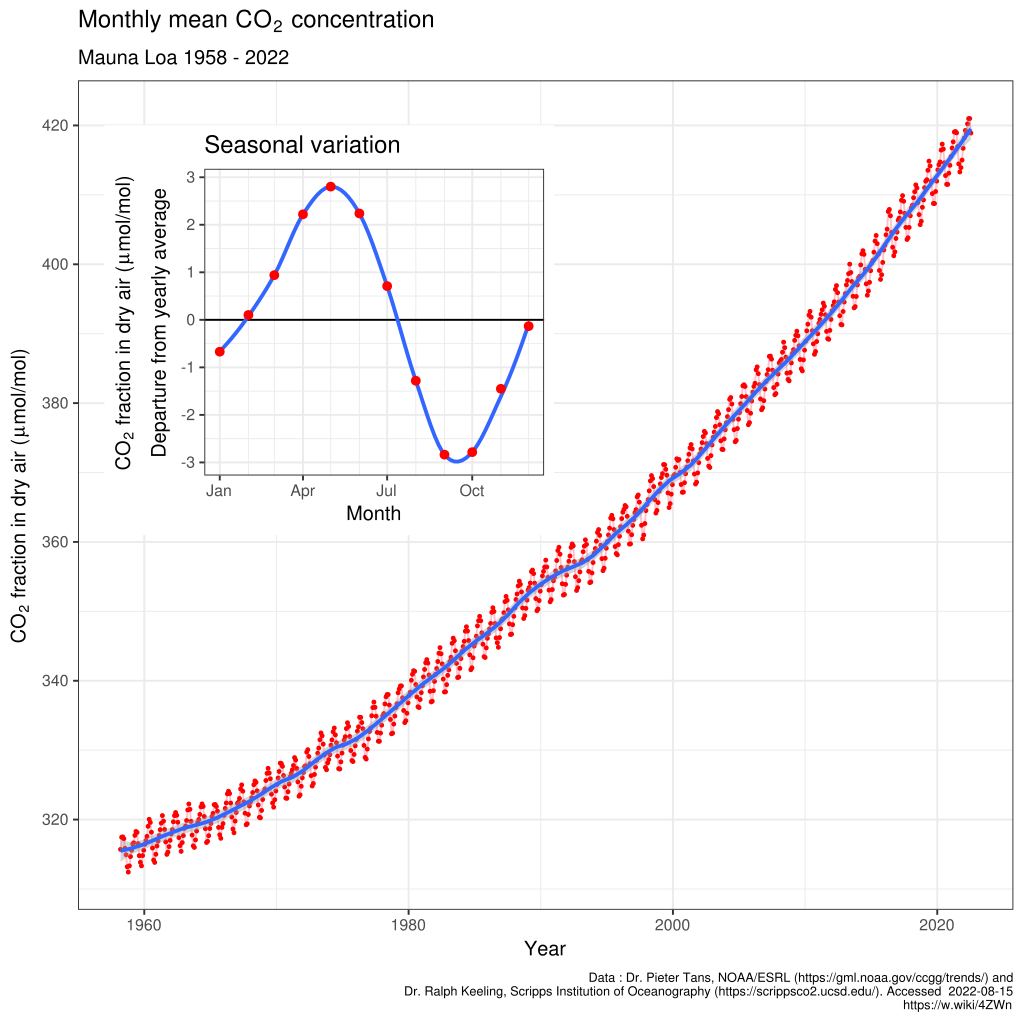
\includegraphics[width=0.3\textwidth]{figures/climate1.png} \hspace{0.5cm}
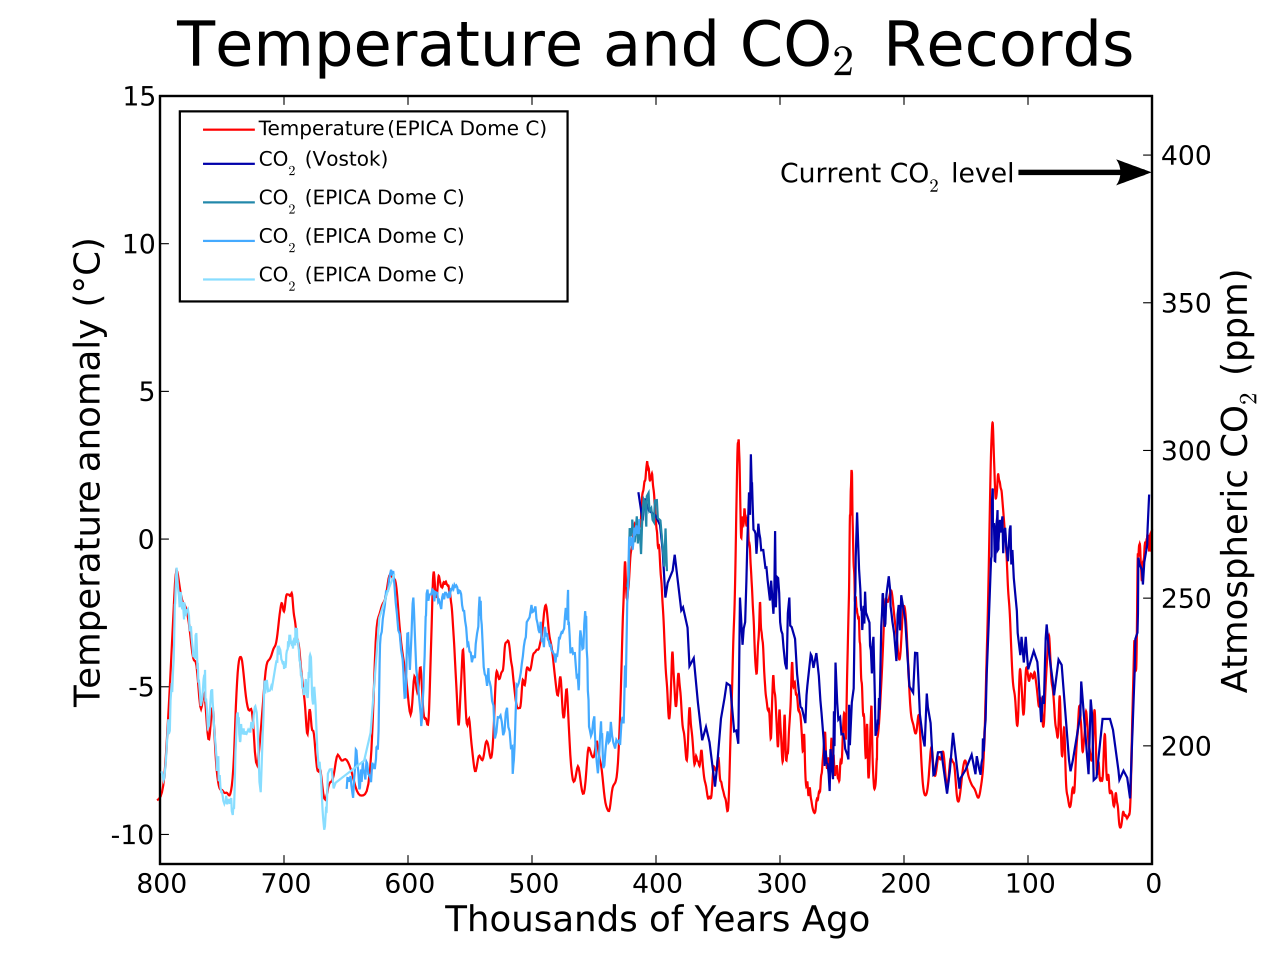
\includegraphics[width=0.3\textwidth]{figures/climate2.png} \hspace{0.5cm}
\caption{\label{fig:1} (Left) Source: ``Inconvenient Truth,'' Wikipedia. (Right) Same as left, Tans and Keeling \textit{et al} from NOAA/ESRL and Scripps Institution of Oceanography.}
\end{figure}

\end{document}
